\chapter{Methodology of Software Development}

\section{Roadmaps and Kanban Boards}
The workflow was effectively managed and visualized using Kanban boards in the project. From initial development phases to final testing, each task was represented by a card on the Kanban board in columns labelled To Do,'' In Progress,'' Testing,'' and Done.'' This method allowed an overview of project progress and fast identification of bottlenecks. Additionally, roadmaps were created to describe the overall strategy and project milestones. These roadmaps defined the steps towards short-term and long-term goals and ensured that development followed the project goals. The Kanban board used for the TrafficVision project can be accessed at \url{https://rohansikder4.atlassian.net/jira/software/projects/KAN/boards/1}, providing a real-time view of project management and task progression.

\begin{figure}[H]
    \centering
    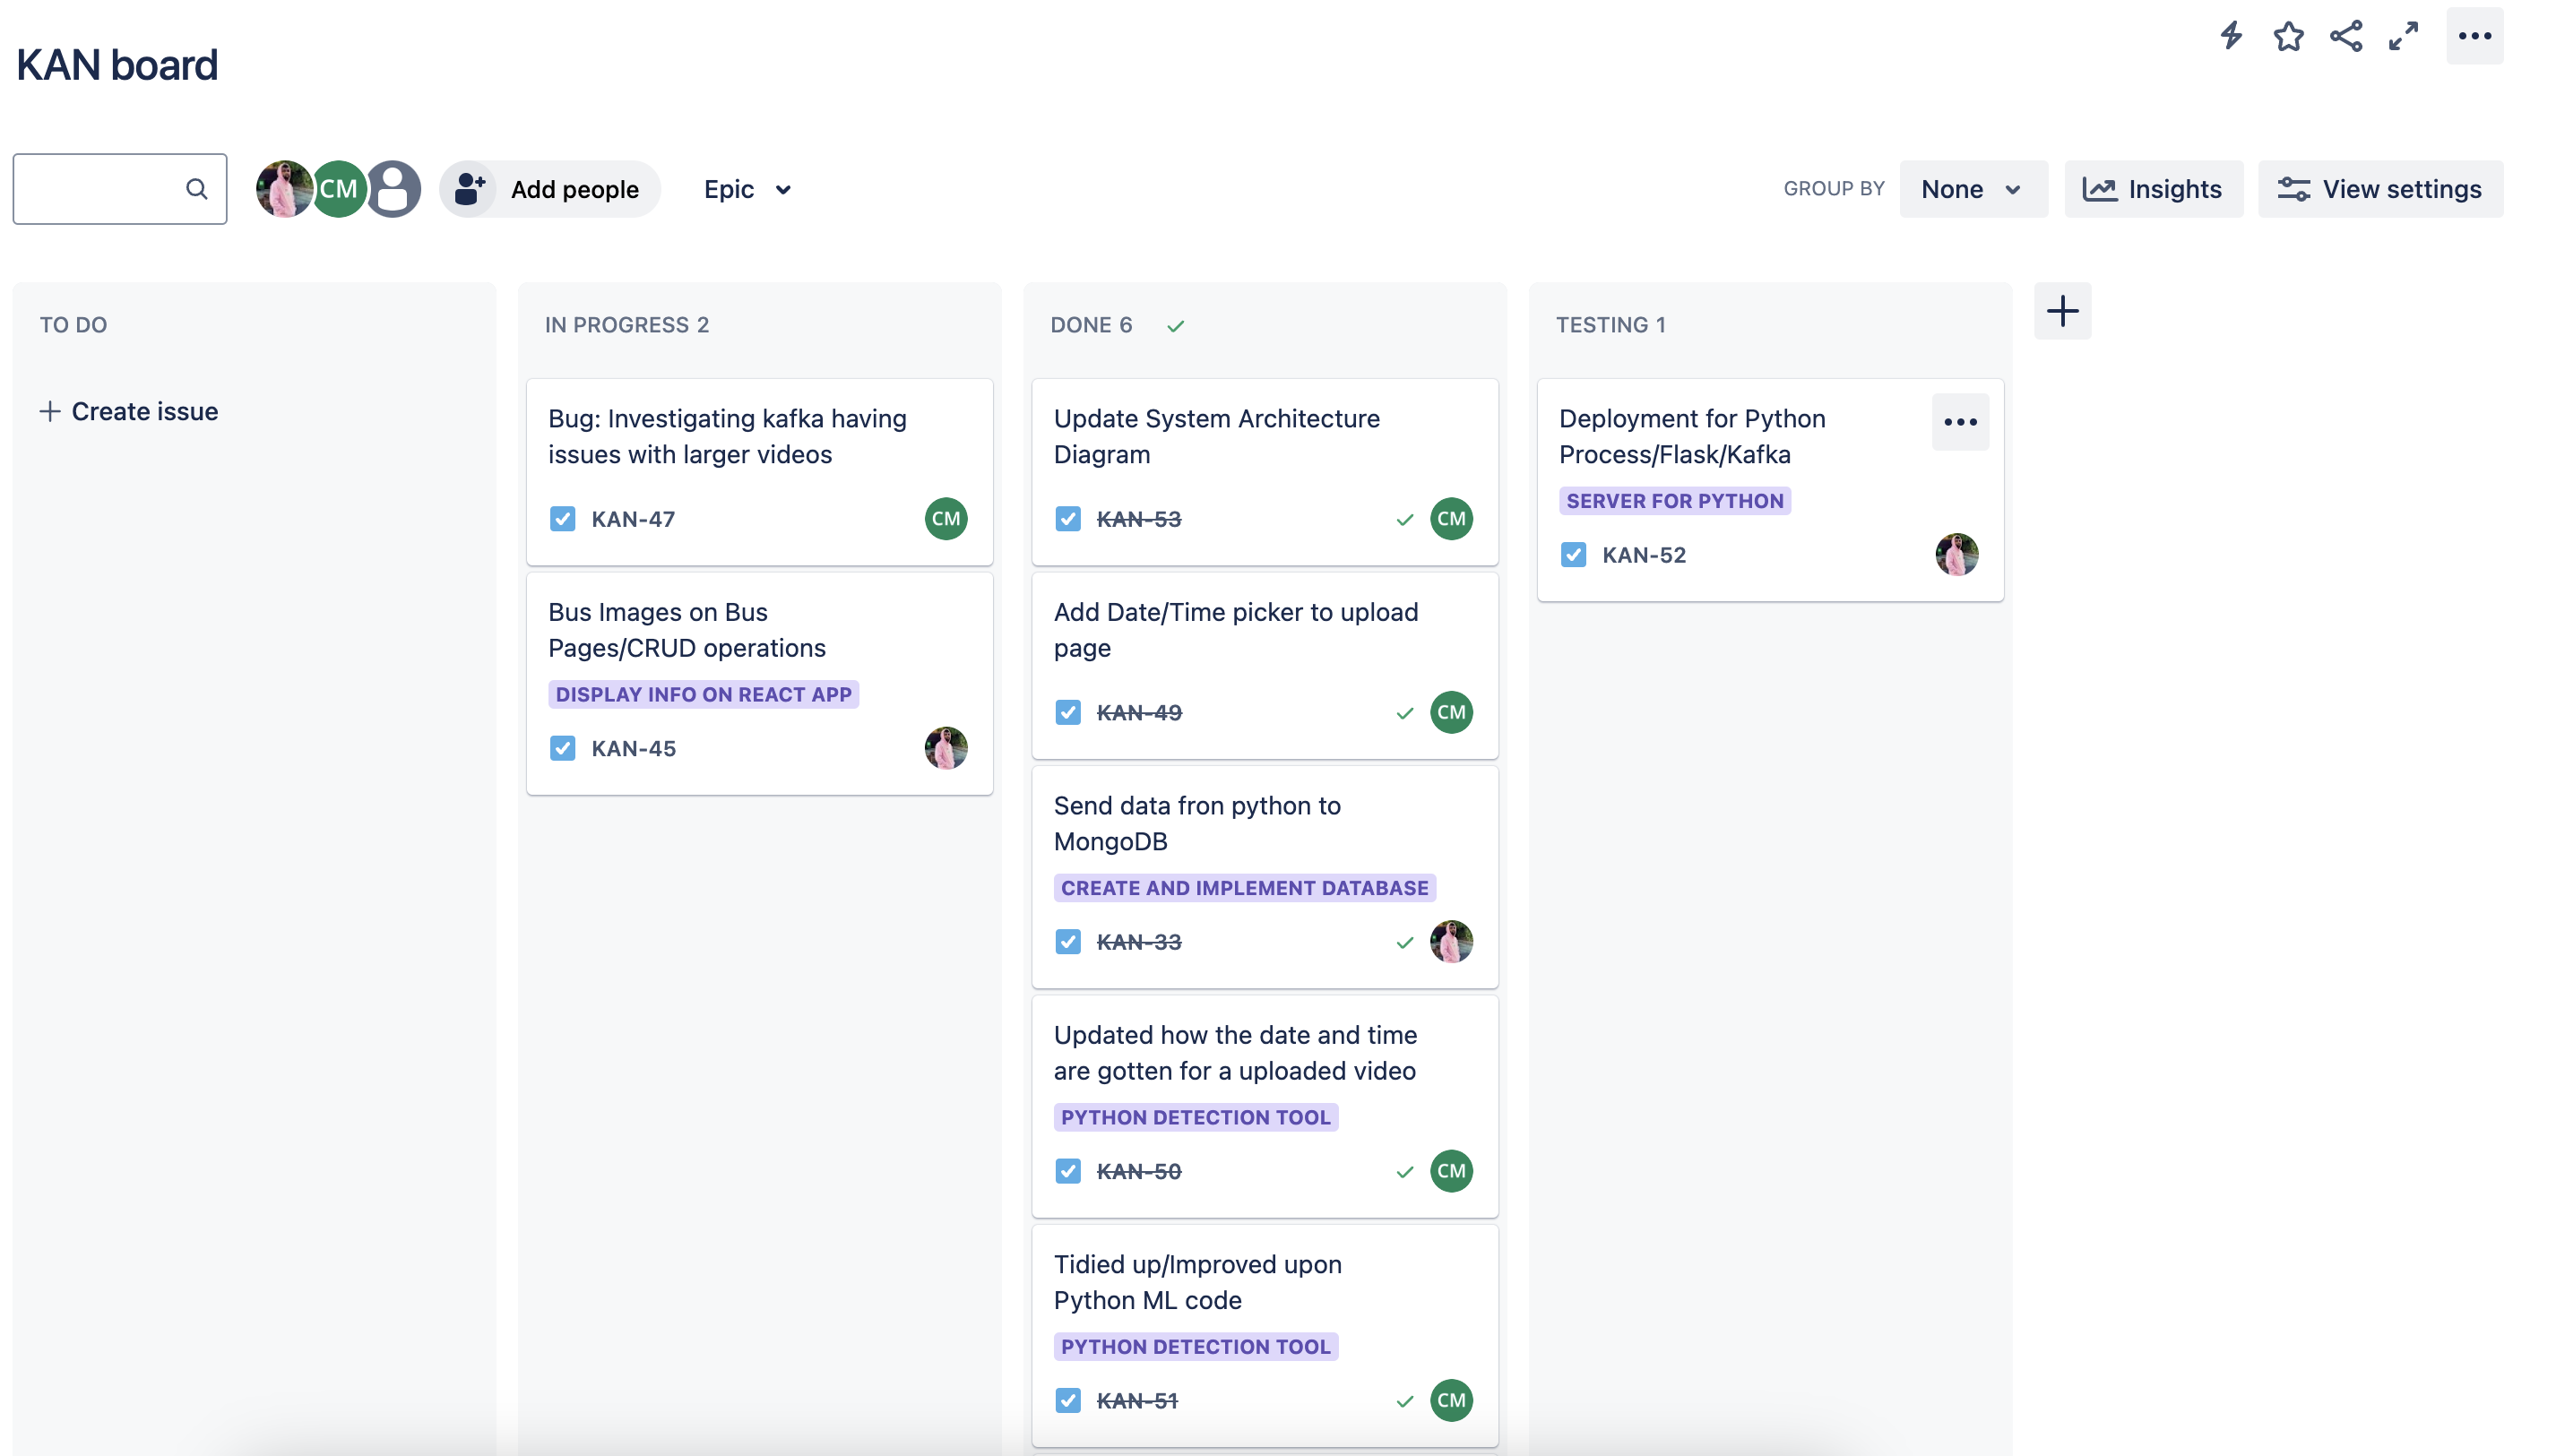
\includegraphics[width=0.8\textwidth]{images/kanban.png}
    \caption{A Screenshot of the Kanban Board.}
    \label{fig:Kanban Board}
\end{figure}


\section{Gantt Chart Integration}
To complement the agile project management approach and enhance visibility into the project timeline, a Gantt chart was employed. This tool was essential in planning, coordinating and tracking specific tasks against time. The Gantt chart for TrafficVision, available at \url{https://rohansikder4.atlassian.net/jira/software/projects/KAN/boards/1/timeline}, illustrates the project’s timeline, including start and end dates for tasks, dependencies and milestones. This visual representation aided in ensuring that project deliverables were completed on schedule and that any potential delays were promptly addressed.


\begin{figure}[h!]
    \centering
    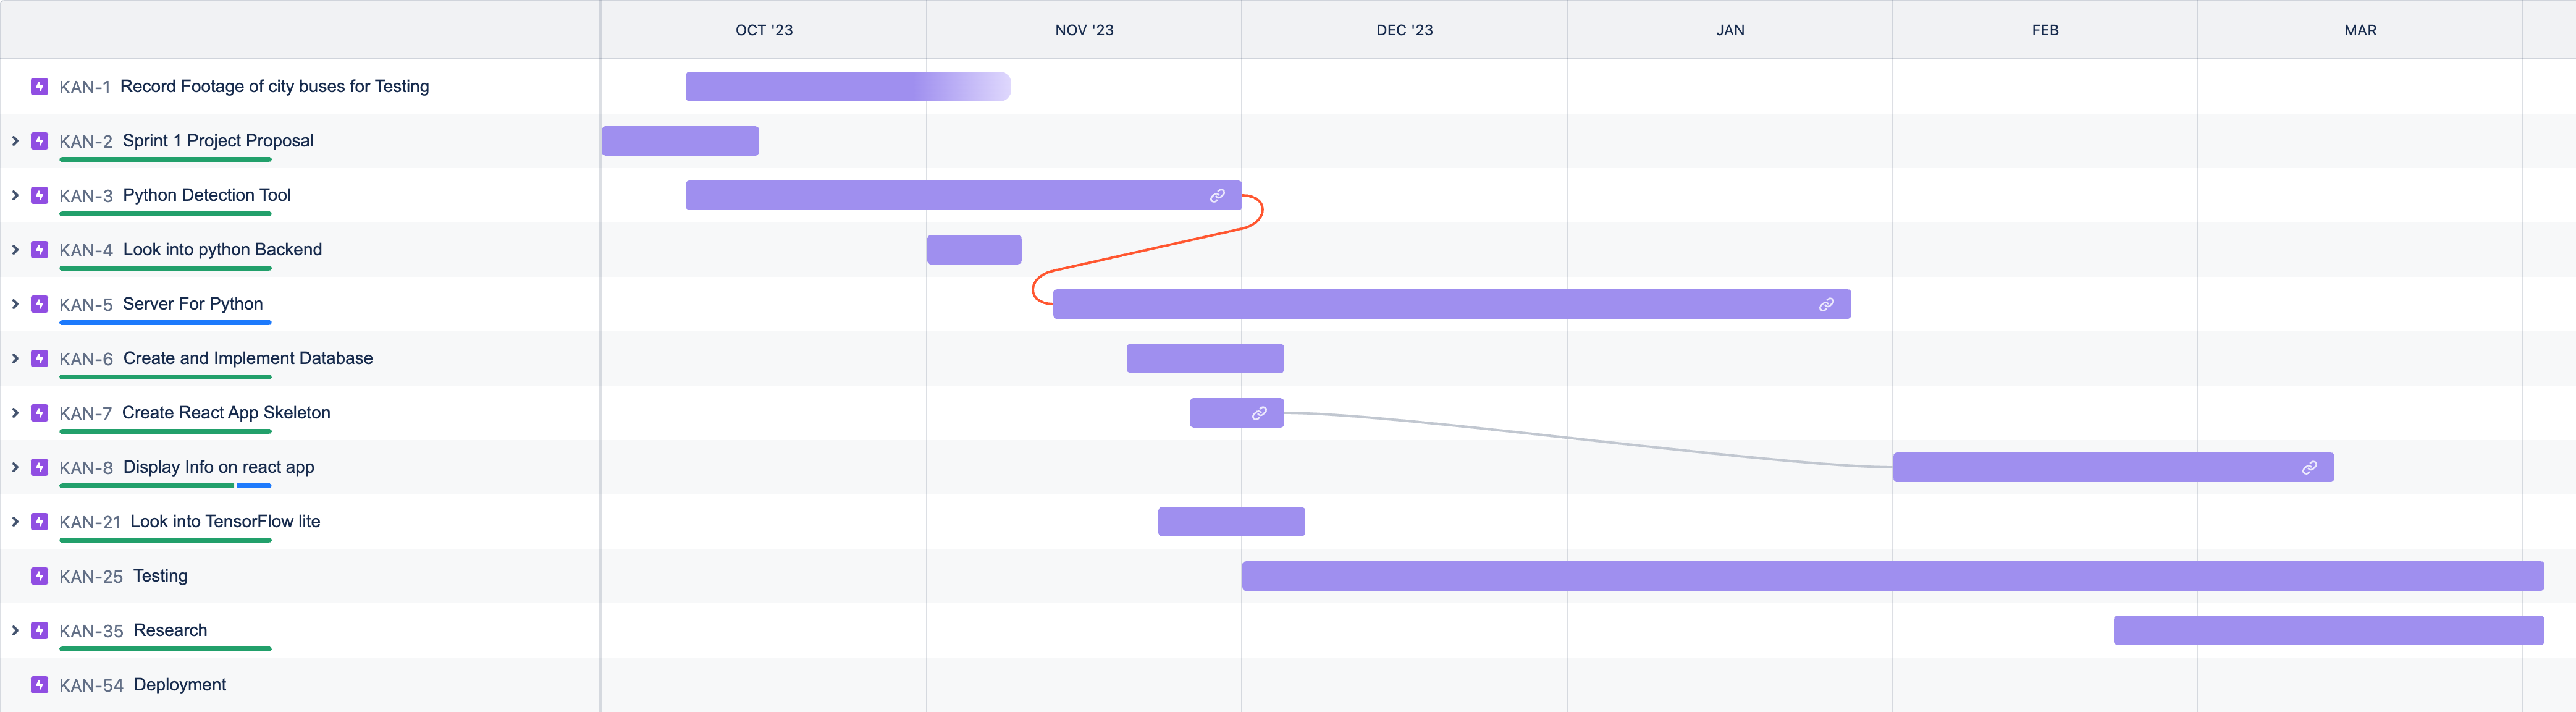
\includegraphics[width=0.8\textwidth]{images/timeline.png}
    \caption{A Gantt Chart which was set out in the beginning of the development proccess.}
    \label{fig:Gantt Chart}
\end{figure}


\section{Agile Methodologies}
While primarily Kanban-based, the project also included elements of Agile\cite{agilemanifesto2001} methodology with emphasis on iterative development and adaptability. Sprint meetings regularly reviewed progress, solved problems and planned future tasks, allowing for rapid iterations on the project scope based on real-time information and feedback.

\section{Meetings and Communication}

Effective communication was essential to the project. Regularly scheduled meetings facilitated continuous project problem-solving and iterative development.

\begin{itemize}
    \item \textbf{Weekly Supervisory Meetings:} Weekly Meetings were held with the project supervisor to review progress and plan future tasks and address immediate issues. These meetings ensured the project met its objectives and offered opportunities for mentorship and guidance. Discussions often revolved around both strategic decisions and technical challenges for a comprehensive project oversight.

    \item \textbf{Weekly Planning Sessions:} Along with supervisory meetings, the team conducted Planning Sessions to outline work for the week. These sessions were critical in clarifying goals, identifying roadblocks and reallocating resources as needed to meet project milestones.

    \item \textbf{Code Review Meetings:} When new Code was written, team members scheduled special Meetings to Review the written Code. These sessions focused on assessing code quality, checking functionality meets project requirements and adding for knowledge sharing and learning. Such reviews helped to maintain high code quality and allowed for group ownership of the project.

    \item \textbf{Issue Resolution Discussions:} Any issues noted during the week or in code reviews were promptly addressed in private discussion sessions. These discussions were essential to troubleshooting issues, brainstorming solutions and delivering fixes on time to avoid project delays.
    
\end{itemize}


\section{Collaboration Tools}
The project used various tools to improve communication and productivity. GitHub\cite{github2024} became the central repository for version control and source code management and was used for reviewing work, facilitating collaboration among team members, regardless of their physical location. This integration of GitHub within the development process underscores its importance as a tool for code collaboration and version control in modern software development.

\section{Rationale for Technology Stack}
The project's choice of MongoDB, Python, React and Node.js as its technology stack was driven by their capabilities to deliver a high-performance web application. Each technology was selected for its strengths in specific areas of the project, from data management to user interface development, ensuring both efficiency and scalability.


\section{Validation and Testing}

Ensuring the quality and reliability of TrafficVision was carried throughout the development process. To achieve this, a comprehensive testing strategy was adopted, employing a mix of manual and automated testing approaches to cover the application's frontend, backend and integration points comprehensively.

\subsection{API Testing with Postman}

Postman\cite{postman2021} was especially important for backend validation, specifically the APIs that execute data transactions between the frontend and the database. A popular API test tool, Postman, allowed to simulate client-side requests to the server and check responses for correctness and performance. By writing structured tests in Postman to ensure all endpoints provided expected functionality, returned appropriate status codes and handled edge cases gracefully. This testing ensured that the server-side logic was robust, fault tolerant and ready to deliver intended user interactions.

\subsubsection{Benefits and Outcomes}
The use of Postman for API testing brought several benefits:
\begin{itemize}
    \item \textbf{Rapid Feedback:} Quick feedback to reduce the time to detect and fix issues.
    \item \textbf{Improved Quality:} Consistent API testing led to higher quality software.
    \item \textbf{Enhanced Reliability:} Load and security testing ensured the APIs could handle real-world usage effectively.
\end{itemize}

\begin{figure}[h!]
    \centering
    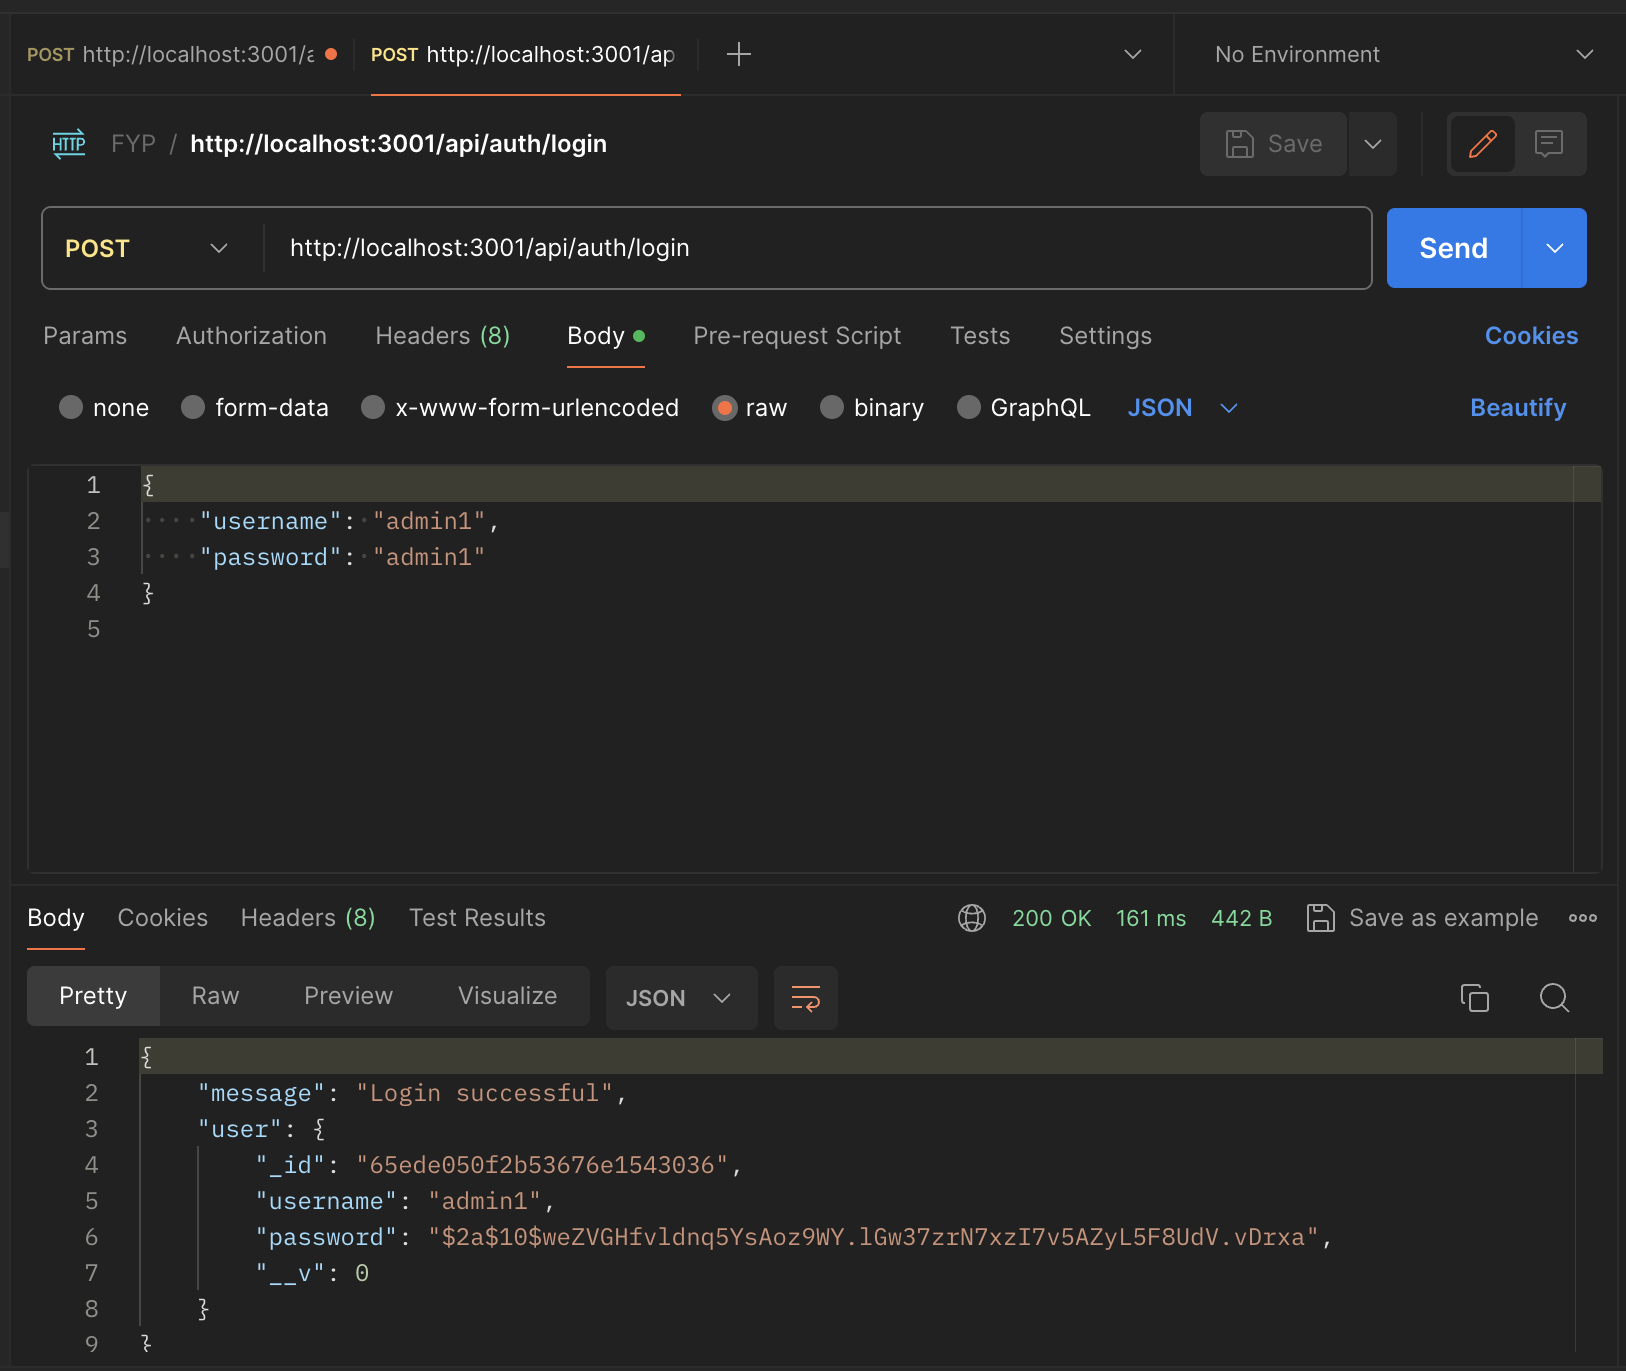
\includegraphics[width=0.8\textwidth]{images/postmanLogin.png}
    \caption{A Postman test demonstrating successful user login API call.}
    \label{fig:postman_login_test}
\end{figure}

\subsection{Developer-Led Frontend Testing}

The frontend was developed with React and tested extensively by the developers that created it. This phase was primarily user testing focusing on the responsiveness, functionality and usability of the user interface. Developers carried out user interactions, navigated the application's features and examined the system behavior in real time. This approach allowed for fast detection and resolution of UI bugs or inconsistencies to ensure intuitive and seamless user experience.

This hands-on testing was complemented by incorporating the frontend and backend services to validate that data flow and processing across system layers worked as intended. This involved testing the real time data display, user authentication and traffic data submission and retrieval.

\subsection{Ensuring Application Robustness}

The combination of Postman for API testing and developers hands-on testing methodology for the frontend meant both critical parts of the TrafficVision application were tested. This methodology allowed for early detection of issues and created quality control.

The project's commitment to testing methodologies emphasized the need to provide a robust and bug-free application capable of enhancing public transportation systems efficiency and reliability. Future enhancements will include additional automated testing frameworks to expand the testing process and coverage to ensure TrafficVision continues to exceed user expectations.

